% !TeX program = lualatex
% !TeX encoding = UTF-8
% !TeX spellcheck = pt_BR

\documentclass[12pt,a4paper]{article}

\usepackage{fontspec}
\defaultfontfeatures{Ligatures=TeX}
\setmainfont{Latin Modern Roman}
\setsansfont{Latin Modern Sans}
\setmonofont{Latin Modern Mono}

\usepackage[brazil]{babel}
\usepackage{csquotes}
\usepackage{geometry}
\geometry{
  top=2.2cm,
  bottom=2.2cm,
  left=1cm,
  right=1cm
}

\usepackage{microtype}
\usepackage{graphicx}
\usepackage{booktabs}
\usepackage{tabularx}
\usepackage{array}
\usepackage{enumitem}
\usepackage{xcolor}
\usepackage{listings}
\usepackage{caption}
\usepackage{xurl}
\usepackage{hyperref}
\usepackage{fancyhdr}
\usepackage{lastpage}

\definecolor{linkblue}{HTML}{1D4ED8}
\definecolor{codegray}{HTML}{F3F4F6}
\definecolor{rulegray}{HTML}{D1D5DB}
\definecolor{commentgreen}{HTML}{166534}
\definecolor{keywordblue}{HTML}{1D4ED8}
\definecolor{stringred}{HTML}{B91C1C}

\hypersetup{
  colorlinks=true,
  linkcolor=linkblue,
  urlcolor=linkblue,
  citecolor=linkblue,
  pdfauthor={Sergio Cordero Calvimontes},
  pdftitle={Relatório técnico do projeto ESP32, MicroPython e OLED SSD1306},
  pdfsubject={Projeto pessoal: processamento assíncrono no ESP32}
}

\pagestyle{fancy}
\fancyhf{}
\lhead{esp32-asyncio}
\rhead{Relatório técnico}
\cfoot{Página \thepage\ de \pageref{LastPage}}
\renewcommand{\headrulewidth}{0.4pt}
\setlength{\headheight}{14.5pt}

\setlist[itemize]{leftmargin=1.5em,itemsep=0.25em,topsep=0.4em}
\setlist[enumerate]{leftmargin=1.7em,itemsep=0.25em,topsep=0.4em}
\setlength{\parindent}{1.2cm}
\setlength{\parskip}{0.25em}
\setlength{\emergencystretch}{2em}

\newcolumntype{Y}{>{\raggedright\arraybackslash}X}
\newcolumntype{C}[1]{>{\centering\arraybackslash}p{#1}}

\lstdefinestyle{pythonstyle}{
  language=Python,
  basicstyle=\small\ttfamily,
  backgroundcolor=\color{codegray},
  frame=single,
  rulecolor=\color{rulegray},
  numbers=left,
  numberstyle=\scriptsize\color{gray},
  numbersep=8pt,
  keywordstyle=\color{keywordblue}\bfseries,
  commentstyle=\color{commentgreen},
  stringstyle=\color{stringred},
  showstringspaces=false,
  breaklines=true,
  columns=fullflexible,
  keepspaces=true,
  tabsize=4,
  xleftmargin=0.6em,
  xrightmargin=0.3em,
  aboveskip=0.8em,
  belowskip=0.8em
}

\lstset{style=pythonstyle}

\newcommand{\ProjectTitle}{Sistema de sinalização com ESP32, LEDs, botão e OLED SSD1306}
\newcommand{\AuthorWebsite}{https://argus-kepheus.github.io/sergio-cordero-calvimontes/\#home}
\newcommand{\AuthorName}{\href{\AuthorWebsite}{Sergio Cordero Calvimontes}}
\newcommand{\WokwiURL}{https://wokwi.com/projects/471528241540407297}
\newcommand{\GitHubURL}{https://github.com/Argus-Kepheus/esp32-asyncio}

\begin{document}

\begin{titlepage}
  \centering
  \vspace*{1.5cm}

  {\Large \textbf{Projeto pessoal}\par}
  \vspace{0.7cm}
  {\large Explorando o processamento assíncrono do ESP32\par}

  \vfill

  {\huge\bfseries \ProjectTitle\par}
  \vspace{0.8cm}
  {\Large Relatório técnico resumido\par}

  \vfill

  \begin{tabular}{rl}
    Autor: & \AuthorName \\
    Plataforma de simulação: & Wokwi \\
    Linguagem: & MicroPython \\
    Placa-alvo: & Espressif ESP32-DevKitC V4 \\
  \end{tabular}

  \vfill

  {\large \today\par}
\end{titlepage}

\tableofcontents
\newpage

\section{Introdução}

Este é um projeto pessoal que explora as capacidades de processamento assíncrono (\texttt{asyncio}) do microcontrolador ESP32. A proposta reúne conteúdos de instrumentação, eletrônica e lógica de programação por meio da simulação de um sistema embarcado baseado em ESP32: seis LEDs azuis piscando de forma assíncrona e independente entre si, um botão pulsador -- um tipo de interruptor que atua apenas enquanto está sendo acionado -- associado a um LED verde, e três mostradores (\textit{displays}) atualizados concorrentemente: dois OLEDs controlados pelo circuito integrado SSD1306, exibindo em tempo real o uso de CPU e de memória RAM, e uma tela TFT ILI9341 funcionando como um console de registro (\textit{log}) colorido.

A simulação executável está publicada no Wokwi em\linebreak[2]
\url{\WokwiURL}. O código-fonte, o diagrama do circuito, a documentação e o histórico de versões estão disponíveis no repositório GitHub em\linebreak[2]
\url{\GitHubURL}.

O Wokwi foi adotado como plataforma principal por oferecer suporte nativo ao ESP32 com MicroPython, edição visual do circuito, arquivo de conexão \texttt{diagram.json}, monitor serial e compartilhamento por endereço eletrônico. O repositório GitHub complementa a simulação ao fornecer rastreabilidade, controle de versões e uma estrutura adequada ao desenvolvimento no Visual Studio Code.

\section{Requisitos e definições do projeto}
\label{sec:requisitos}

\subsection{Requisitos funcionais e estados do sistema}

O sistema satisfaz seus requisitos funcionais por meio de várias tarefas independentes, executadas concorrentemente sob escalonamento cooperativo (\texttt{asyncio}): uma tarefa por LED azul, uma tarefa que relaciona o botão ao LED verde, duas tarefas indicadoras do estado do sistema (barramento e escalonador) e uma tarefa de atualização para cada um dos três mostradores.

\begin{description}
  \item[Seis LEDs azuis, seis tarefas independentes:] Cada um dos seis LEDs (GPIO~26, 14, 27, 25, 33 e 12) alterna seu próprio estado em uma tarefa \texttt{asyncio} própria, sem depender de nenhuma outra tarefa nem ser bloqueado por ela. Todos compartilham um mesmo intervalo, ajustável em tempo real por dois botões dedicados (GPIO~34 diminui, GPIO~35 aumenta) que escalam o intervalo de todos os seis simultaneamente pelo mesmo fator. Na teoria, isso mantém os seis sincronizados entre si; na prática, essa sincronia é apenas nominal. Por serem tarefas independentes, cada uma mede sua própria pausa a partir do instante em que retoma a execução, e não a partir de um relógio absoluto compartilhado -- pequenos atrasos causados por outras tarefas (sobretudo as escritas bloqueantes nos mostradores) se acumulam de forma diferente em cada LED a cada ciclo. Após alguns minutos de operação contínua, torna-se perceptível a dessincronização visual entre os seis, independentemente do intervalo configurado no momento. Essa dessincronização não é um defeito de implementação, e sim uma limitação inerente ao escalonamento cooperativo: nada garante que tarefas nominalmente idênticas permaneçam em fase entre si indefinidamente.

  \item[Botão e LED verde:] Lê o botão conectado ao GPIO~17, com antirrepique por software, e reflete o estado estável no LED verde (GPIO~4): \textbf{solto} desliga o LED, \textbf{pressionado} liga o LED. Cada transição é registrada no console da tela TFT, em verde. Pelo mesmo motivo da dessincronização acima, a amostragem do botão compete por tempo de processamento com as demais tarefas assíncronas; em alguns instantes -- tipicamente quando uma escrita bloqueante nos mostradores está em andamento -- é necessário manter o botão pressionado por mais tempo que o nominal para que a janela de estabilidade de 30~[ms] do antirrepique seja efetivamente acumulada, já que ciclos de amostragem podem ser adiados enquanto o processador está ocupado.

  \item[LED laranja -- barramento ocupado:] Fica aceso por padrão e apaga apenas durante as escritas bloqueantes nos mostradores (\texttt{show()} / \texttt{fill\_rect()}), funcionando como um indicador invertido de \enquote{\textit{bus busy}}: apagado significa que o barramento I\textsuperscript{2}C ou SPI está, naquele instante, efetivamente ocupado transferindo dados.

  \item[LED amarelo -- escalonador ocioso:] Liga somente quando nenhuma outra tarefa tem trabalho pendente naquele instante, funcionando como indicador de quão ocioso está o escalonador cooperativo -- análogo a uma tarefa de prioridade mínima em um sistema operacional de tempo real.

  \item[Mostrador de uso de CPU (primeiro OLED):] Atualizado a cada 250~[ms] com a fração real do tempo gasto em transferências I\textsuperscript{2}C/SPI bloqueantes desde a última amostra -- um substituto medido para \enquote{uso de CPU}, já que o MicroPython no ESP32 não expõe essa métrica diretamente.

  \item[Mostrador de uso de RAM (segundo OLED):] Atualizado a cada 250~[ms] com o uso real de memória do coletor de lixo do MicroPython (\texttt{gc.mem\_alloc()} / \texttt{gc.mem\_free()}), em um barramento I\textsuperscript{2}C independente do primeiro OLED.

  \item[Console de registro (tela TFT):] Recebe, de forma assíncrona e a partir de várias tarefas diferentes, linhas de texto coloridas sobre os eventos do sistema -- uma cor por subsistema -- rolando pela tela como um registro (\textit{log}) de atividade.
\end{description}

A atualização periódica dos três mostradores não serve apenas para exibir informação: sua função também é manter o processador deliberadamente ocupado, evitando que fique ocioso por longos períodos. É justamente essa carga que torna visíveis, através dos LEDs laranja e amarelo descritos acima, os instantes reais de ocupação e ociosidade do sistema -- e é essa mesma disputa por tempo de processamento que explica tanto a dessincronização dos LEDs azuis quanto a eventual necessidade de segurar o botão por mais tempo.

\subsection{Definições de hardware}

A placa selecionada foi a \textbf{Espressif ESP32-DevKitC V4}, representada no Wokwi pelo componente \texttt{board-esp32-devkit-c-v4}. A especificação original exige apenas \enquote{MicroPython para ESP32}; portanto, a escolha da placa não decorre de uma necessidade exclusiva de desempenho. Ela foi assumida por ser uma placa oficial da Espressif, documentada, identificada de forma inequívoca no simulador e capaz de disponibilizar todos os GPIOs requeridos. A Tabela \ref{tab:pinagem} apresenta a pinagem específica adotada para este projeto.

Para eventual montagem física, recomenda-se uma ESP32-DevKitC V4 equipada com módulo ESP32-WROOM, preferencialmente ESP32-WROOM-32E. Versões com módulo WROVER devem ser evitadas sem revisão do projeto, pois GPIO~16 e GPIO~17 podem ser reservados para a memória PSRAM.

Além da placa selecionada, outras placas de desenvolvimento poderiam ser utilizadas sem problemas de compatibilidade de pinos, desde que baseadas no chip ESP32 (arquitetura Xtensa LX6) com módulo WROOM -- e não WROVER, S2, S3, C3 ou C6, cujos mapeamentos de GPIO, reservas de memória e conjunto de periféricos diferem do exigido por este projeto. Entre as alternativas compatíveis estão:

\begin{itemize}
  \item Espressif ESP32-DevKitC V2, a revisão anterior da placa adotada, com o mesmo módulo ESP32-WROOM-32 e cabeçalho (\textit{header}) de 38 pinos;
  \item placas genéricas \enquote{NodeMCU-32S} (ESP-WROOM-32), amplamente disponíveis de diversos fabricantes, com layout de 38 pinos equivalente;
  \item \enquote{DOIT ESP32 DevKit V1}, com módulo ESP32-WROOM-32 em cabeçalho de 30 pinos, desde que os GPIOs~26, 4, 16, 17 e 32 estejam expostos;
  \item Clones com módulo WROOM-32 de fabricantes como AZ-Delivery ou HiLetgo, que replicam o mesmo mapeamento de GPIOs do módulo original.
\end{itemize}

Em todos os casos, é necessário confirmar que os GPIOs~16 e 17 não estão reservados para PSRAM ou outra função interna do módulo específico antes de reutilizar o mapeamento de pinos deste projeto.

\begin{table}[htbp]
  \centering
  \caption{Pinagem completa do projeto, agrupada por subsistema.}
  \label{tab:pinagem}
  \begin{tabularx}{\textwidth}{@{}Y C{1.5cm} C{2.2cm} Y@{}}
    \toprule
    Função & GPIO & Terminal físico$^{1}$ & Identificador no código \\
    \midrule
    \multicolumn{4}{@{}l}{\textit{LEDs piscantes -- seis tarefas independentes, todos azuis (\texttt{\#0000FF}) no circuito atual$^{2}$}} \\
    LED piscante 1 & 26 & J2-10 & \texttt{red\_led} / \texttt{RED\_LED\_PIN} \\
    LED piscante 2 & 14 & J2-12 & \texttt{blue\_led} / \texttt{BLUE\_LED\_PIN} \\
    LED piscante 3 & 27 & J2-11 & \texttt{yellow\_led} / \texttt{YELLOW\_LED\_PIN} \\
    LED piscante 4 & 25 & J2-9 & \texttt{white\_led} / \texttt{WHITE\_LED\_PIN} \\
    LED piscante 5 & 33 & J2-8 & \texttt{orange\_led} / \texttt{ORANGE\_LED\_PIN} \\
    LED piscante 6 & 12 & J2-13 & \texttt{red\_led\_2} / \texttt{RED\_LED\_2\_PIN} \\
    \midrule
    \multicolumn{4}{@{}l}{\textit{Botão principal e LED verde}} \\
    Botão pulsador principal & 17 & J3-11 & \texttt{push\_button} / \texttt{BUTTON\_PIN} \\
    LED verde (indicador do botão) & 4 & J3-13 & \texttt{green\_led} / \texttt{GREEN\_LED\_PIN} \\
    \midrule
    \multicolumn{4}{@{}l}{\textit{Botões de controle de velocidade}} \\
    Botão -- diminuir intervalo & 34 & J2-5 & \texttt{decrease\_speed\_button} \\
    Botão -- aumentar intervalo & 35 & J2-6 & \texttt{increase\_speed\_button} \\
    \midrule
    \multicolumn{4}{@{}l}{\textit{LEDs indicadores de estado do sistema}} \\
    LED laranja -- barramento ocupado & 13 & J2-15 & \texttt{bus\_idle\_led} \\
    LED amarelo -- escalonador ocioso & 2 & J3-15 & \texttt{scheduler\_idle\_led} \\
    \midrule
    \multicolumn{4}{@{}l}{\textit{Primeiro OLED -- mostrador de uso de CPU, barramento I\textsuperscript{2}C(0)}} \\
    Relógio I\textsuperscript{2}C (SCL) & 32 & J2-7 & \texttt{OLED\_SCL\_PIN} \\
    Dados I\textsuperscript{2}C (SDA) & 16 & J3-12 & \texttt{OLED\_SDA\_PIN} \\
    \midrule
    \multicolumn{4}{@{}l}{\textit{Segundo OLED -- mostrador de uso de RAM, barramento I\textsuperscript{2}C(1) independente}} \\
    Relógio I\textsuperscript{2}C (SCL) & 15 & J3-16 & \texttt{OLED2\_SCL\_PIN} \\
    Dados I\textsuperscript{2}C (SDA) & 22 & J3-3 & \texttt{OLED2\_SDA\_PIN} \\
    \midrule
    \multicolumn{4}{@{}l}{\textit{Tela TFT -- console de registro, SPI genuíno de 4 fios}} \\
    Relógio SPI (SCK) & 18 & J3-9 & \texttt{TFT\_SCK\_PIN} \\
    Dados de saída SPI (MOSI) & 23 & J3-2 & \texttt{TFT\_MOSI\_PIN} \\
    Seleção de circuito (CS) & 5 & J3-10 & \texttt{TFT\_CS\_PIN} \\
    Dado/comando (D/C) & 21 & J3-6 & \texttt{TFT\_DC\_PIN} \\
    Reinicialização (RST) & 19 & J3-8 & \texttt{TFT\_RST\_PIN} \\
    \midrule
    Chave deslizante de modo de gravação$^{3}$ & 0 & J3-14 & -- \\
    \bottomrule
  \end{tabularx}

  \vspace{0.3em}
  \raggedright\footnotesize
  $^{1}$Identificação do conector (J2 ou J3) e da posição do terminal no cabeçalho físico de 38 pinos da ESP32-DevKitC V4, conforme \texttt{docs/EN/hardware-reference.md}.\\
  $^{2}$Os identificadores de código (\texttt{red\_led}, \texttt{yellow\_led}, \texttt{white\_led}, \texttt{orange\_led}, \texttt{red\_led\_2}) são nomes herdados de uma fase anterior do projeto, quando cada LED tinha uma cor física distinta planejada. No circuito atual todos os seis LEDs piscantes são fisicamente azuis; o nome de cada variável no código serve apenas para diferenciá-la das demais, não para descrever a cor real do componente.\\
  $^{3}$Lida apenas pelo \textit{bootloader} ROM do ESP32 antes de qualquer script MicroPython iniciar; nenhum código de \texttt{main.py} interage com ela.
\end{table}

O primeiro LED piscante (GPIO~26) e o relógio I\textsuperscript{2}C do primeiro OLED (GPIO~32) foram realocados dos GPIO~2 e GPIO~25, originalmente fixados antes do início do desenvolvimento, a pedido explícito do usuário, por motivos de layout da placa à medida que mais periféricos foram adicionados (ver o registro de decisões em \texttt{docs/EN/technical-specification.md}, §16). O GPIO~2 liberado foi posteriormente reaproveitado pelo LED indicador amarelo do escalonador, e o GPIO~25 pelo quarto LED piscante -- a Tabela~\ref{tab:pinagem} reflete a fiação atual, não a atribuição original.

A numeração utilizada corresponde aos números dos GPIOs do microcontrolador e não à posição sequencial dos terminais físicos da placa; a coluna ``Terminal físico'' indica exatamente essa posição sequencial, para referência ao montar o circuito fisicamente. Todos os LEDs possuem resistores limitadores de 220~[$\Omega$], e todos os componentes compartilham a mesma referência de terra.

\subsection{Entrada do botão e antirrepique}
\label{sec:antirrepique}

O GPIO~17 é configurado como entrada com resistor interno de redução (\textit{pull-down}). Dessa forma, o terminal permanece em nível baixo com o botão aberto e passa ao nível alto quando o contato conecta o GPIO à alimentação de 3,3~[V].

Essa configuração dispensa a implementação física de um resistor de \textit{pull-down} externo: o próprio microcontrolador disponibiliza esse resistor internamente, ativado por software (\texttt{Pin.PULL\_DOWN}), o que simplifica o circuito, reduz o número de componentes e elimina uma fonte de erro de montagem.

Os dois botões de controle de velocidade (GPIO~34 e GPIO~35, Tabela~\ref{tab:pinagem}) não podem usar essa mesma facilidade: são pinos exclusivamente de entrada e não dispõem de nenhum resistor interno de redução ou de elevação (\textit{pull-up}). Por isso, cada um desses dois botões utiliza um resistor externo de \textit{pull-down} de 10~[k$\Omega$], já incluído em \texttt{diagram.json}, reproduzindo o mesmo comportamento solto~=~LOW / pressionado~=~HIGH do botão principal.

Não foi acrescentado filtro RC externo em nenhum dos três botões. O antirrepique (\textit{bouncing}) é realizado por programa, sem bloqueio: o nível é amostrado periodicamente e uma alteração somente é aceita quando permanece estável por aproximadamente 30~[ms]. Essa estratégia é suficiente para a aplicação e evita oscilações do LED verde e atualizações repetidas do OLED.

Essas duas medidas fazem sentido sobretudo para uma implementação física: um botão pulsador mecânico real produz múltiplas transições elétricas espúrias durante o acionamento, e é esse ruído que o antirrepique elimina. O simulador Wokwi, por outro lado, modela o botão como um interruptor ideal, sem esse ruído de contato. Na simulação, portanto, o antirrepique não é estritamente necessário e é mantido apenas como boa prática, de modo que o mesmo código já esteja correto caso o projeto seja migrado para um botão físico sem qualquer alteração de lógica.

\subsection{Interface dos três mostradores}
\label{sec:mostrador-interface}

Os três mostradores do sistema usam duas interfaces de comunicação diferentes, cada uma escolhida pela natureza do tráfego que efetivamente precisa suportar.

Os dois OLEDs SSD1306 se comunicam por I\textsuperscript{2}C, cada um em seu próprio barramento de hardware independente (\texttt{machine.I2C(0)} e \texttt{machine.I2C(1)}), de modo que ambos podem ser endereçados ao mesmo tempo sem disputa de barramento. O primeiro usa GPIO~32 como relógio (SCL) e GPIO~16 como dados (SDA); o segundo usa GPIO~15 (SCL) e GPIO~22 (SDA). O endereço adotado para os dois é \texttt{0x3C}, com resolução de 128 por 64~[pixels] cada. A utilização de I\textsuperscript{2}C para o primeiro OLED foi definida antes da etapa de desenvolvimento -- o enunciado original exigia apenas que um mostrador refletisse o estado do botão, sem especificar interface ou pinos --, e, uma vez definida, foi tratada como fixa e reaplicada ao segundo OLED quando este foi adicionado, para manter a mesma interface nos dois mostradores monocromáticos. A interface I\textsuperscript{2}C usa apenas dois sinais de comunicação por barramento e é adequada às atualizações periódicas, porém pouco frequentes (a cada 250~[ms]), dos dois gráficos de uso de CPU e RAM (Seção~\ref{sec:oled-graphs}).

A tela TFT ILI9341, por sua vez, usa SPI genuíno de 4 fios -- relógio (SCK), dados de saída (MOSI), seleção de circuito (CS) e dado/comando (D/C), além de uma linha independente de reinicialização (RST) --, em GPIO~18, 23, 5, 21 e 19 respectivamente, com resolução de 240 por 320~[pixels] e cor de 16 bits (RGB565). Diferentemente dos dois OLEDs, a TFT funciona como um console de registro (\textit{log}) colorido (Seção~\ref{sec:tft-console}) que recebe uma nova linha de texto a cada evento relevante do sistema -- uma frequência de atualização bem maior e mais irregular que a dos dois gráficos de uso de CPU/RAM. SPI oferece maior taxa de transferência que I\textsuperscript{2}C à custa de mais sinais de controle, o que se justifica aqui pelo volume de dados que esse console efetivamente movimenta, bem maior que as mensagens estáticas do enunciado original.

\section{Desenvolvimento do programa \texttt{main.py}}

\subsection{Estrutura geral}

O arquivo \texttt{main.py} concentra a inicialização do hardware e a coordenação das tarefas.

Uma organização representativa da aplicação é mostrada a seguir:

\begin{lstlisting}[caption={Estrutura lógica resumida do programa.},label={lst:estrutura}]
BLINKING_LEDS = [
    [red_led, RED_LED_BLINK_INTERVAL_MS],
    [blue_led, BLUE_LED_BLINK_INTERVAL_MS],
    [yellow_led, YELLOW_LED_BLINK_INTERVAL_MS],
    [white_led, WHITE_LED_BLINK_INTERVAL_MS],
    [orange_led, ORANGE_LED_BLINK_INTERVAL_MS],
    [red_led_2, RED_LED_2_BLINK_INTERVAL_MS],
]

async def blink_led(entry):
    """Toggle one LED at its own interval, independent of every other task."""
    led, _ = entry
    while True:
        led.value(not led.value())
        await asyncio.sleep_ms(entry[1])

async def monitor_button(initial_state):
    """React to every debounced push-button transition."""
    await debounce_button(push_button, initial_state, apply_button_state)

async def main():
    initial_button_state = bool(push_button.value())
    apply_button_state(initial_button_state)

    for entry in BLINKING_LEDS:
        asyncio.create_task(blink_led(entry))
    asyncio.create_task(scheduler_idle_task())
    asyncio.create_task(update_cpu_graph())
    asyncio.create_task(update_ram_graph())
    asyncio.create_task(print_status())
    asyncio.create_task(
        monitor_step_button(decrease_speed_button, lambda: apply_blink_speed_step(-1))
    )
    asyncio.create_task(
        monitor_step_button(increase_speed_button, lambda: apply_blink_speed_step(+1))
    )
    await monitor_button(initial_button_state)
\end{lstlisting}

Este trecho é uma síntese da arquitetura; o código completo e executável está disponível no repositório.

\subsection{Assincronismo cooperativo}

A biblioteca \texttt{asyncio} do MicroPython foi escolhida como arquitetura exclusiva do projeto. Em vez de um superlaço (\textit{superloop}) que verifica manualmente diversos temporizadores, cada função independente pode ser organizada como uma corrotina (\textit{coroutine}). A instrução \texttt{await asyncio.sleep\_ms(...)} suspende apenas a tarefa atual e devolve o controle ao escalonador (\textit{scheduler}).

Essa decisão foi tomada pelos seguintes motivos:

\begin{itemize}
  \item Separação clara entre o piscar de cada LED, a leitura de cada botão e a atualização de cada mostrador;
  \item Menor acoplamento entre funcionalidades e facilidade de manutenção e escalabilidade;
  \item Prevenção de congelamentos causados por \texttt{time.sleep()} no fluxo principal;
  \item Melhor tolerância às pequenas latências introduzidas pela transmissão por meio do barramento I\textsuperscript{2}C.
\end{itemize}

O assincronismo adotado é cooperativo. Portanto, as tarefas devem alcançar pontos de espera com frequência e evitar rotinas longas ou bloqueantes.

\subsection{LEDs piscantes e controle de velocidade}

O sistema controla seis LEDs piscantes independentes (Tabela~\ref{tab:pinagem}), todos fisicamente azuis no circuito atual. Em vez de uma corrotina escrita à mão para cada LED, \texttt{main.py} mantém uma única lista, \texttt{BLINKING\_LEDS}, com um par \texttt{[objeto Pin, intervalo em milissegundos]} por LED, e lança uma tarefa \texttt{blink\_led()} idêntica para cada par dessa lista, em um laço \texttt{for} (Código~\ref{lst:estrutura}). Cada par é uma lista mutável, não uma tupla, porque o intervalo é reescrito em tempo real pelos botões de velocidade enquanto a tarefa correspondente já está em execução: \texttt{blink\_led()} relê \texttt{entry[1]} a cada ciclo, em vez de capturá-lo uma única vez no início, permitindo que uma mudança de velocidade tenha efeito imediato sem reiniciar nenhuma tarefa.

Os dois botões de controle de velocidade (GPIO~34 diminui, GPIO~35 aumenta -- Seção~\ref{sec:antirrepique}) alteram a velocidade dos seis LEDs de uma só vez: cada pressão desloca, em uma unidade, um fator de escala em potência de dois aplicado sobre o intervalo-base de 500~[ms] de cada LED, limitado a um intervalo mínimo de 125~[ms] e máximo de 4~[s]. A cada mudança, o novo intervalo é registrado no console da TFT em azul (Seção~\ref{sec:tft-console}).

\subsection{Botão principal, LED verde e console de registro}

O botão principal (GPIO~17) e os dois botões de velocidade compartilham a mesma corrotina genérica de antirrepique, \texttt{debounce\_button()}: ela amostra o pino periodicamente, aguarda 30~[ms] de estabilidade (Seção~\ref{sec:antirrepique}) e só então invoca uma função de retorno (\textit{callback}) específica para cada botão. Para o botão principal, essa função é \texttt{apply\_button\_state()}: liga ou desliga o LED verde (GPIO~4) conforme o novo estado estável e registra a transição no console da TFT, em verde.

Diferentemente da versão original deste projeto, nenhum OLED recebe mais uma mensagem de texto associada ao botão -- essa responsabilidade foi completamente substituída pelo console de registro da TFT, já que os dois OLEDs passaram a ser gráficos de uso de CPU e RAM (Seção~\ref{sec:oled-graphs}) sem espaço livre para texto adicional. Caso a TFT não tenha sido detectada na inicialização, \texttt{apply\_button\_state()} também imprime a mesma mensagem no console serial, para que uma falha de fiação da TFT não silencie por completo a realimentação de estado do botão.

\subsection{Indicadores de barramento ocupado e escalonador ocioso}
\label{sec:idle-leds}

Dois LEDs adicionais tornam visível, em tempo real, um comportamento interno do escalonador cooperativo que de outra forma não teria nenhuma manifestação observável no circuito.

O LED laranja (GPIO~13, \texttt{bus\_idle\_led}) permanece aceso por padrão e apaga apenas durante uma escrita bloqueante em algum dos três mostradores. Um par de funções auxiliares, \texttt{\_bus\_busy\_begin()} e \texttt{\_bus\_busy\_end()}, encapsula toda chamada bloqueante de \texttt{show()}/\texttt{fill\_rect()}/\texttt{text()} nos três mostradores: apaga o LED no início da chamada, mede sua duração real com \texttt{time.ticks\_us()} e o acende de volta ao final -- acumulando essa mesma duração em \texttt{bus\_busy\_time\_us}, consumida pelo gráfico de uso de CPU (Seção~\ref{sec:oled-graphs}).

O LED amarelo (GPIO~2, \texttt{scheduler\_idle\_led}) liga e desliga em uma tarefa própria, \texttt{scheduler\_idle\_task()}, sem nenhum compromisso de tempo fixo: a cada iteração ela apenas alterna o LED e devolve o controle ao escalonador com \texttt{await asyncio.sleep\_ms(0)}, o menor atraso possível. Como o \texttt{asyncio} do MicroPython não implementa níveis reais de prioridade entre tarefas, essa tarefa só recebe tempo de processamento nos intervalos em que nenhuma outra tarefa tem trabalho pendente naquele instante -- funcionando, portanto, como uma aproximação grosseira de uma tarefa de prioridade mínima (\textit{idle task}) de um sistema operacional de tempo real, não uma implementação literal de uma. Uma vez por segundo, essa mesma tarefa também registra no console da TFT, em amarelo, quantas iterações desse laço conseguiu completar no último segundo -- uma medida aproximada de quanta capacidade de processamento sobra além do que as demais tarefas já consomem.

\subsection{Mostradores de uso de CPU e RAM (dois OLEDs)}
\label{sec:oled-graphs}

Os dois OLEDs SSD1306 não exibem mais nenhuma mensagem de texto estática: cada um foi convertido em um gráfico de barras rolante, no estilo de um monitor de tarefas, atualizado a cada 250~[ms] (\texttt{update\_cpu\_graph()} e \texttt{update\_ram\_graph()}). Cada amostra ocupa uma coluna de pixels na largura do OLED (até 128 amostras de histórico); ao atingir o limite, a amostra mais antiga é descartada e todas as colunas são redesenhadas a cada janela.

O primeiro OLED plota um substituto medido para "uso de CPU": como o MicroPython no ESP32 não expõe nenhuma métrica de carga de um escalonador de sistema operacional, o valor plotado é, em vez disso, a fração real de cada janela de amostragem gasta dentro de uma transferência I\textsuperscript{2}C/SPI bloqueante -- acumulada via \texttt{bus\_busy\_time\_us} (Seção~\ref{sec:idle-leds}) --, já que essa é a única situação em que esta aplicação de núcleo único e escalonamento cooperativo está de fato ocupada executando, em vez de suspensa em um ponto de espera (\texttt{await}). A janela de amostragem em si é medida com \texttt{time.ticks\_us()}, não assumida como exatamente 250~[ms]: \texttt{asyncio.sleep\_ms()} garante apenas um atraso mínimo, e uma chamada mais lenta a \texttt{console\_log()} em outra tarefa pode empurrar o intervalo real bem além do solicitado -- dividir pelo intervalo assumido, quando mais curto que o real, foi a causa de uma leitura defeituosa acima de 100\% observada durante os testes e desde então corrigida.

O segundo OLED plota o uso real de memória do coletor de lixo do MicroPython (\texttt{gc.mem\_alloc()} / \texttt{gc.mem\_free()}), em seu próprio barramento I\textsuperscript{2}C independente (Seção~\ref{sec:mostrador-interface}).

\subsection{Console de registro colorido (TFT)}
\label{sec:tft-console}

A tela TFT funciona como um console de registro (\textit{log}) rolante, no estilo do \texttt{dmesg} de um sistema Unix ou do histórico de instalação de um gerenciador de pacotes: cada evento do sistema imprime uma linha de texto colorida; ao preencher a última linha visível, a próxima linha volta para o topo da tela (não há rolagem real de conteúdo -- ver \texttt{console\_log()} em \texttt{main.py}). Cada cor está associada a um subsistema e, sempre que esse subsistema tem um LED físico correspondente, à mesma cor desse LED:

\begin{itemize}
  \item Azul -- os seis LEDs piscantes;
  \item Verde -- o botão principal e o LED verde;
  \item Laranja -- o LED indicador de barramento ocupado;
  \item Amarelo -- o LED indicador de escalonador ocioso;
  \item Vermelho -- o gráfico de uso de CPU;
  \item Roxo/lilás -- o gráfico de uso de RAM;
  \item Branco -- mensagens gerais, sem um subsistema colorido correspondente (inicialização, diagnósticos de falha).
\end{itemize}

A implementação de texto (\texttt{ili9341.py}, método \texttt{text()}) foi otimizada após um levantamento de desempenho: a versão original convertia cada glifo em pixels individuais por meio de \texttt{framebuf.FrameBuffer.pixel()}, chamada até cerca de 1920 vezes por linha de texto. A versão atual pré-calcula, uma única vez por combinação de cor de texto e cor de fundo, uma tabela de conversão de 256 entradas -- uma por valor de byte possível -- para os 16 bytes RGB565 correspondentes a essa fatia de 8 pixels do glifo, e reutiliza essa tabela a cada caractere renderizado, eliminando o laço pixel a pixel do caminho crítico. Do mesmo modo, \texttt{console\_log()} evita limpar a linha inteira do console a cada mensagem: apenas o trecho da linha além da largura real do texto é apagado (\texttt{fill\_rect()}), já que \texttt{text()} já pinta sua própria cor de fundo sob cada caractere que desenha.

\section{Estratégia de verificação e testes isolados}
\label{sec:testes}

O desenvolvimento foi acompanhado por testes progressivos. A separação dos subsistemas permitiu distinguir erros de ligação, inicialização e lógica de aplicação.

\begin{enumerate}
  \item \textbf{Teste isolado do primeiro LED piscante:} Utilizou um laço bloqueante mínimo somente para diagnóstico. O GPIO~26 foi alternado a cada 500~[ms] e o estado foi registrado no monitor serial. O objetivo foi confirmar placa, pino, resistor, polaridade e retorno ao terra sem interferência das demais funções.

  \item \textbf{Teste do mesmo LED com o idioma de alternância:} Repetiu o teste anterior usando \texttt{led.value(not led.value())}, o mesmo idioma de alternância de nível que \texttt{blink\_led()} efetivamente usa em \texttt{main.py}, ainda em um laço bloqueante, sem \texttt{asyncio} -- isolando essa mudança de estilo de código como uma variável independente da introdução do \texttt{asyncio} no teste seguinte.

  \item \textbf{Teste do mesmo LED com \texttt{asyncio}:} Repetiu o teste anterior, agora encapsulado em uma corrotina agendada com \texttt{asyncio.create\_task()} dentro de \texttt{asyncio.run()}, isolando especificamente o suporte a \texttt{asyncio} do firmware como variável, separado da fiação e do idioma de alternância já confirmados.

  \item \textbf{Teste isolado do botão e do LED verde:} Amostrou o GPIO~17 periodicamente e refletiu o estado lido no GPIO~4, sem qualquer dependência de nenhum LED piscante ou do OLED. O objetivo foi confirmar a fiação do botão, o resistor interno de redução e o comportamento ativo em nível alto isoladamente.

  \item \textbf{Teste básico do OLED:} Inicializou o barramento I\textsuperscript{2}C em GPIO~32 e GPIO~16, confirmou a detecção do endereço \texttt{0x3C} por meio de \texttt{i2c.scan()} e apresentou uma mensagem simples.

  \item \textbf{Diagnóstico gráfico do SSD1306:} Exercitou todos os pixels ligados e desligados, padrões quadriculados complementares, varreduras horizontais e verticais, grade, pixels individuais, linhas, retângulos, áreas preenchidas, texto, inversão, contraste, desligamento, religamento e deslocamento do quadro.

  \item \textbf{Teste básico dos LEDs extras:} Verificou, um de cada vez e com um laço bloqueante mínimo, a fiação dos cinco LEDs piscantes adicionais (GPIO~14, 27, 25, 33 e 12), no mesmo espírito do teste 1.

  \item \textbf{Seis LEDs piscantes concorrentes:} Reuniu o LED do teste 1--3 e os cinco LEDs do teste 7 rodando ao mesmo tempo, cada um em sua própria tarefa \texttt{asyncio}, exatamente como \texttt{BLINKING\_LEDS} em \texttt{main.py}.

  \item \textbf{Botões de velocidade:} Validou os dois botões pulsadores adicionais (GPIO~34 e GPIO~35) e seus resistores externos de \textit{pull-down}, diferentemente do resistor interno usado pelo botão principal no teste 4.

  \item \textbf{LEDs indicadores:} Validou a fiação dos dois LEDs indicadores de estado do sistema -- laranja de barramento ocupado (GPIO~13) e amarelo de escalonador ocioso (GPIO~2).

  \item \textbf{Segundo OLED:} Validou o segundo barramento I\textsuperscript{2}C independente (\texttt{I2C(1)}, GPIO~15/22) do segundo OLED, isolado do barramento do primeiro.

  \item \textbf{TFT básica:} Validou a fiação SPI de 4 fios da TFT (SCK~18, MOSI~23, CS~5, D/C~21) e sua linha de reinicialização (RST~19): inicialização do painel e preenchimentos de cor sólida.

  \item \textbf{Diagnóstico de texto da TFT:} Exercitou o método \texttt{text()} de \texttt{ili9341.py} -- a primitiva sobre a qual o console de registro de \texttt{main.py} é construído -- em todas as cores usadas pelo console, incluindo o retorno ao topo da tela ao preencher todas as linhas visíveis.
\end{enumerate}

A sequência de testes reduziu o espaço de busca de falhas: se um subsistema simples não funcionasse, o problema poderia ser tratado antes da integração com o restante da aplicação. A tabela de dependências completa entre os treze testes, e uma recomendação de subconjunto mínimo (\textit{smoke test}) para quando não há tempo de rodar todos, estão em \texttt{tests/README.md}.

\section{Circuito simulado}
\label{sec:circuito}

A Figura~\ref{fig:circuito} apresenta o estado atual do circuito no Wokwi. Com o número maior de componentes e sinais, as cores dos condutores no diagrama deixaram de seguir uma convenção única por função; a pinagem completa e atual de todo o projeto está na Tabela~\ref{tab:pinagem} (Seção~\ref{sec:requisitos}).

\begin{figure}[htbp]
  \centering
  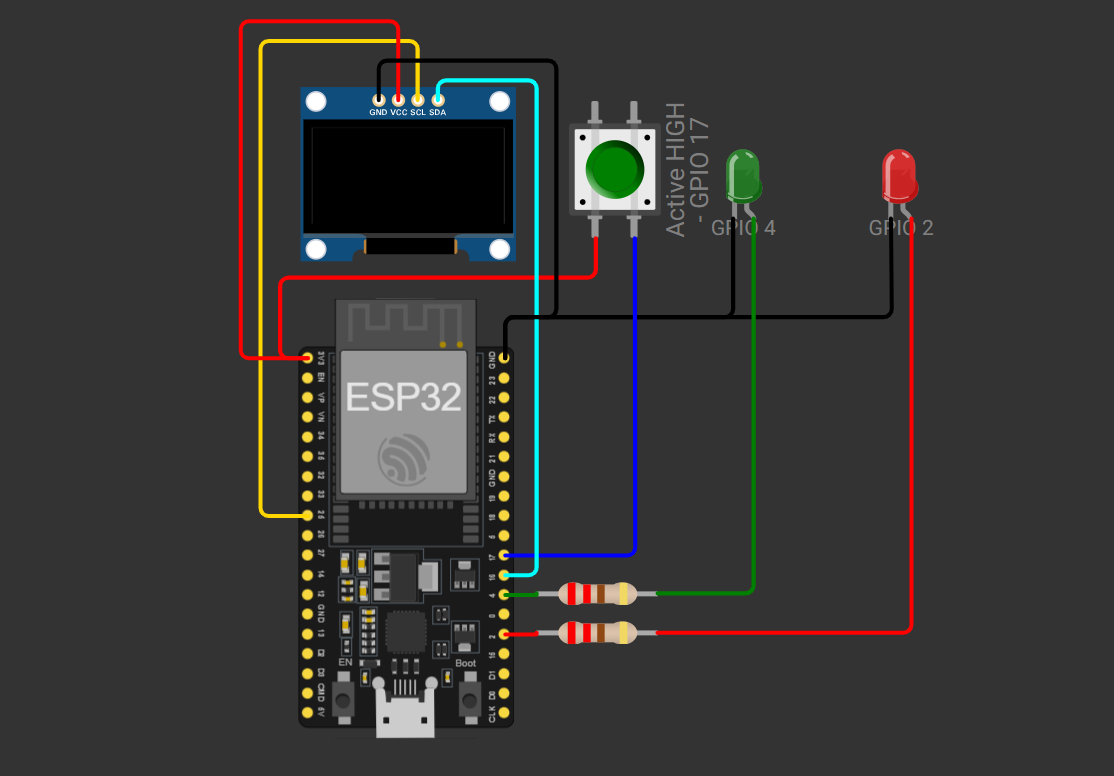
\includegraphics[
    width=0.72\textwidth,
    height=0.475\textheight,
    keepaspectratio
  ]{figures/circuito-wokwi.png}
  \caption{Circuito do projeto no Wokwi: ESP32-DevKitC V4, dois OLEDs SSD1306, display TFT ILI9341, seis LEDs azuis, um LED verde, dois LEDs indicadores de estado (laranja e amarelo), três botões pulsadores e uma chave deslizante.}
  \label{fig:circuito}
\end{figure}

\section{Conclusão}

O projeto atende aos requisitos definidos por meio de uma implementação modular e reproduzível. A escolha da ESP32-DevKitC V4 reduz ambiguidades de pinagem, enquanto o uso explícito de cada GPIO (Tabela~\ref{tab:pinagem}) preserva a correspondência entre código, documentação e circuito. As duas interfaces de comunicação adotadas -- I\textsuperscript{2}C para os dois OLEDs e SPI de 4 fios para a TFT -- atendem adequadamente à natureza distinta do tráfego de cada mostrador, conforme discutido na Seção~\ref{sec:mostrador-interface}.

A arquitetura assíncrona permite a concorrência de seis tarefas de LED, duas tarefas indicadoras de estado, três tarefas de atualização de mostrador e o monitoramento de três botões, sem que nenhuma delas bloqueie as demais. O antirrepique compartilhado elimina a necessidade de filtro externo nesta aplicação e em suas três variantes de botão, e as otimizações aplicadas ao console de registro da TFT -- tabela de conversão de cor pré-calculada, limpeza apenas do trecho residual de cada linha -- mantêm o tempo de escrita bloqueante baixo o suficiente para não dominar o próprio gráfico de uso de CPU que ele ajuda a alimentar. Por fim, os treze testes isolados e progressivos (Seção~\ref{sec:testes}) forneceram evidências de funcionamento de cada subsistema antes da integração completa.

A entrega é complementada por dois meios de acesso: a simulação pública no Wokwi e o repositório versionado no GitHub. Em conjunto, eles possibilitam executar, inspecionar, reproduzir e evoluir o projeto.

\section*{Referências eletrônicas}
\addcontentsline{toc}{section}{Referências eletrônicas}

\begin{itemize}
  \item Projeto no Wokwi: \url{\WokwiURL}
  \item Repositório no GitHub: \url{\GitHubURL}
  \item Guia da ESP32-DevKitC V4: \url{https://docs.espressif.com/projects/esp-dev-kits/en/latest/esp32/esp32-devkitc/user_guide.html}
  \item MicroPython para ESP32: \url{https://docs.micropython.org/en/latest/esp32/quickref.html}
  \item Documentação da \texttt{asyncio}: \url{https://docs.micropython.org/en/latest/library/asyncio.html}
  \item Componente SSD1306 do Wokwi: \url{https://docs.wokwi.com/parts/board-ssd1306}
\end{itemize}

\end{document}